%\chapter{Preliminaries}
\chapter{実験1 -色度による光沢感変化-}

    \section{目的}
        実験1では,輝度は同一であるが色度のみが異なる刺激に対して知覚される光沢感を測定する.
        色度ごとの光沢感を定量化することで,光沢感に色度情報が寄与しているかどうかを明らかにすることを目的とする.

        \subsection{作業仮説}
            第1章で述べたとおり,物体の表面の輝度成分が光沢感知覚に寄与していることは既知である.
            しかし,輝度が変わると当然知覚的な明るさも変わるため,光沢感に寄与しているのが知覚的な明るさ感なのか輝度情報そのものなのかについては明らかになっていない.

            本実験で検証する仮説は,拡散反射成分と鏡面反射成分の知覚的な明るさ感のコントラストが主に光沢感に寄与しているというものである.
            鏡面反射成分と拡散反射成分の色度情報を利用して明るさ感のみを変化させれば,輝度の効果と明るさの効果を分離できる.
            これを利用し,反射成分を拡散反射成分と鏡面反射成分に分け,拡散反射成分のみについて輝度を一定に保ったまま色度を変化させ有彩色を付与する処理を行う.
            このとき,もし上述の仮説が正しいとすれば,H-K効果による明るさ感の増幅が顕著な色度では,拡散反射成分の明るさ感がH-K効果により向上することに起因し,他色度に比べて相対的に明るさ感のコントラストが大きく減少するため,光沢感が小さくなるはずである.
            また,コントロール刺激として拡散反射成分と鏡面反射成分の両方に輝度を変えずに色度を変化させた刺激を用意する.
            この刺激は拡散反射成分と鏡面反射成分の両方の明るさ感がH-K効果により向上するため,ハイライトの明るさのコントラストについて色度による変化が生じない.
            明るさ感のコントラストが光沢感知覚に寄与しているならば,この2種類の刺激に対する色度の影響が異なるはずである.

    \section{実験方法}
        \subsection{被験者}
            本実験は20代男性7人に対して行われた.
            全被験者の視力または矯正視力は正常であり,かつ石原式色覚異常検査表により色覚が正常であることが確認されていた.

        \subsection{実験環境}

            \begin{figure}[h]
                \centering
                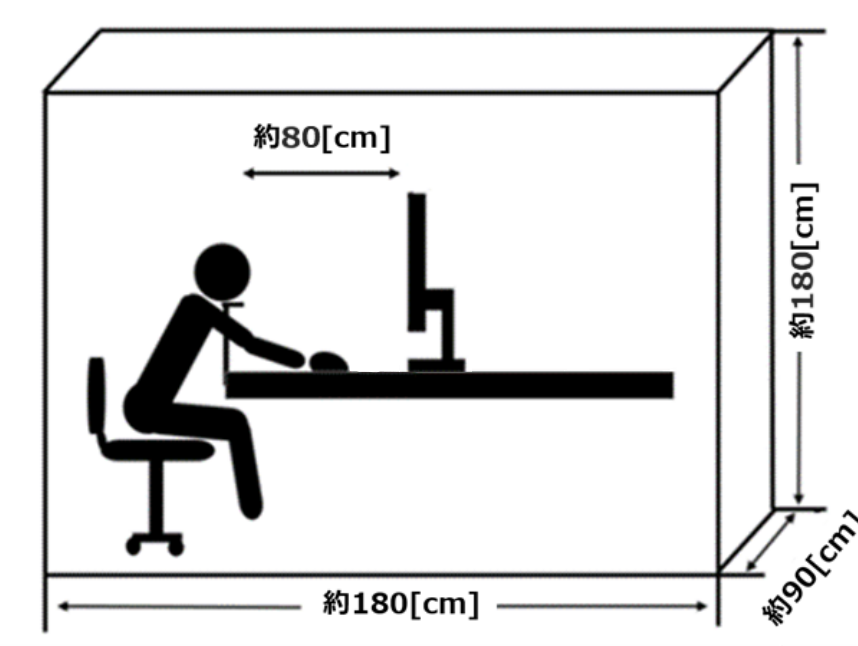
\includegraphics[width=10.0cm]{./img/darkroom_p.png}
                \caption{実験環境概略図}
                \label{darkroom}
            \end{figure}
            
            図\ref{darkroom}に実験環境の概略図を示す.
            暗幕で覆われた簡易的な暗室内に刺激呈示用液晶ディスプレイ(EIZO社 ColorEdge CS2420,解像度 1920ピクセル$\times$1200ピクセル,リフレッシュレート60Hz)を設置し実験を行った.
            また,刺激の輝度と色度を正確に投影するために分光反射輝度計 (Cambridge Research Systems 社 SpectroCAL) によりモニタの分光分布を,色彩輝度計(Cambridge Research Systems 社 ColorCAL2)によりモニタのガンマ特性を測定した.
            これにより,所望のCIE $XYZ$三刺激値をモニタに呈示することが可能となった.
            
            実験はすべてPC(DELL 社 Vostro 13 5000,OS: Ubuntu 18.04.3 LTS)で統制され,MathWorks MATLABとPsychtoolbox3\cite{Psychtoolbox}を用いてプログラムを作成・実行することでディスプレイの刺激呈示と被験者応答を管理した.
            実験中,被験者の頭部はディスプレイから80cmの距離に顎台により固定され,両眼自然視でディスプレイを観察した.
            被験者はトラックボールマウスを使用して応答した.

        \subsection{実験刺激}

            \begin{figure}[h]
                \centering
                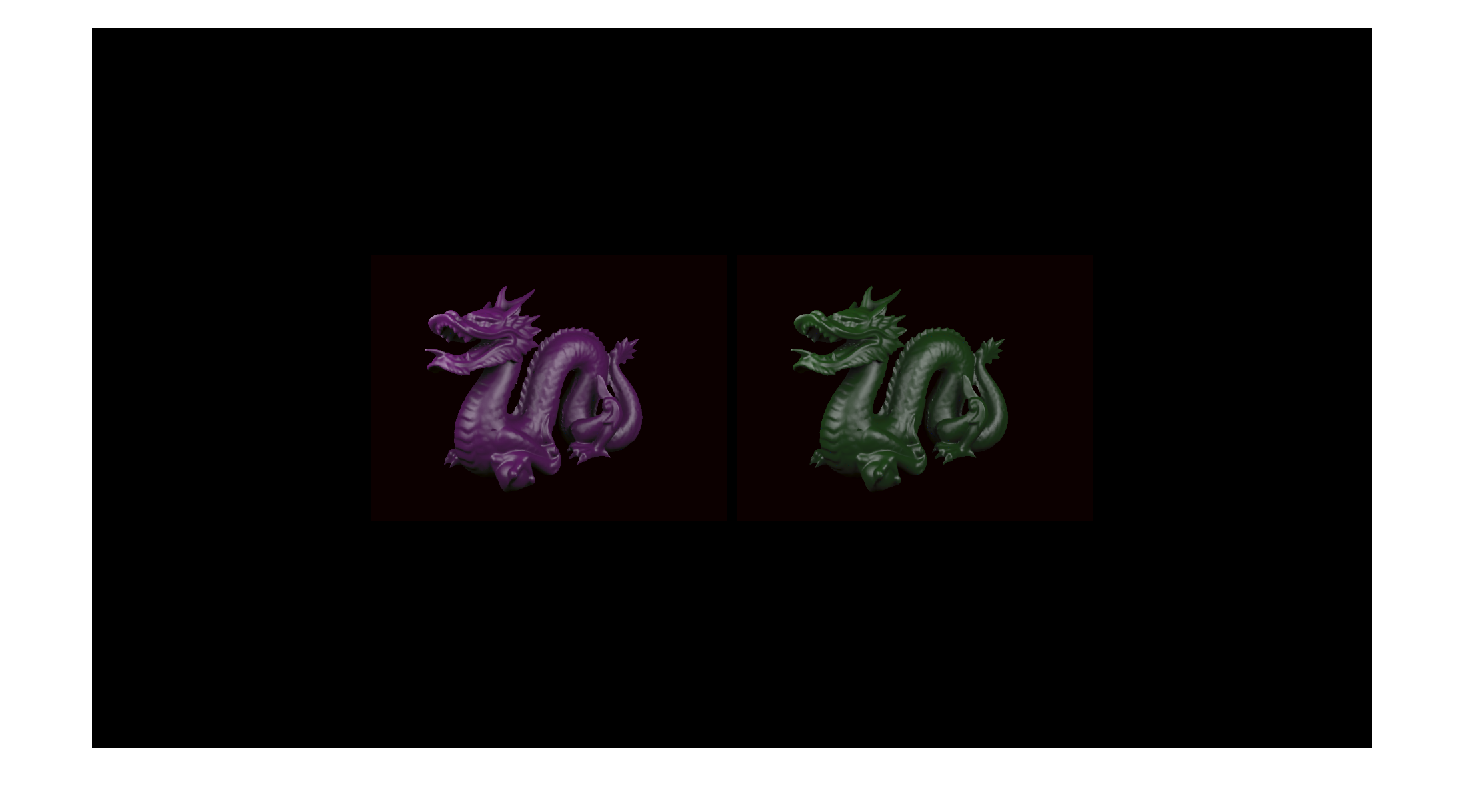
\includegraphics[width=14.0cm]{./img/ex1_stimuli.png}
                \caption{実験刺激の例}
                \label{ex1_stimuli}
            \end{figure}

            図\ref{ex1_stimuli}に実験1で使用する刺激の例を示す.
            刺激は黒背景上の中心部分の縦6.42deg,横17.35degの範囲の左右に呈示される二枚のコンピュータグラフィックス画像であった.
            これらの画像はモニタ中央を挟んで対称な位置に呈示された.
            また,各画像はコンピュータグラフィックスソフトウェアを用いたレンダリングと,MATLAB上での簡易的な画像処理を用いた彩色という,二つの工程を経て作られた.
            以下の節に,これらの工程の詳細を記す.

            \subsubsection{レンダリング}
                実験に用いた刺激の元となる無彩色刺激は RenderToolbox4 によって,レンダラーを Mitsuba\cite{Mitsuba} として作成された.
                この際の照明環境はCIE標準光源D65であり,物体の分光反射率は全波長にわたり同じ値であった.
                物体形状として,Stanford Dragon と Stanford Bunny \cite{StanfordModels} の2種類を使用し,照明環境も含めた環境のジオメトリはBlender 2.79により設定した.
                一方,表面反射特性は RenderToolbox4 と Mitsuba により設定し,その反射モデルとしてWardモデル\cite{Ward}を用いた.
                この際,拡散反射成分と鏡面反射成分の色度を別々に操作するため,これらの反射成分は独立にレンダリングされた.
                このレンダリングにおけるパラメータを表\ref{render_param}に示す.

                \begin{table}[h]
                    \centering
                    \caption{レンダリング時のパラメータ}
                    \begin{tabular}{|l||c|c|c|} \hline
                                               & SpecularReflectance & DiffuseReflectance & Roughness \\ \hline \hline
                        拡散反射成分           & 0                   & 0.1                & 0.2 \\ \hline
                        鏡面反射成分           & 0.9                 & 0                  & 0.2 \\ \hline
                    \end{tabular}
                    \label{render_param}
                \end{table}
            
            \subsubsection{彩色}
                レンダリングされた画像は上述したとおりD65の色度を持つ画像であったが,その画像に対して色条件を設定するために色度を付与した.
                その方法はSD彩色とD彩色の2種類であった.
                SD彩色では,拡散反射成分と鏡面反射成分の両方に同じ色度を設定し,それらのCIE $XYZ$値を加算して作成した.
                D彩色では,拡散反射成分にのみ色度を付与した一方で,鏡面反射成分の色度はD65の値のまま変化させず,それらの$XYZ$値を加算して作成した.
                彩色において,レンダリングされた画像そのものはHDR画像であり,非常に高輝度な領域を含む画像であった.
                しかし,モニタが呈示可能な輝度の最大値はせいぜい100${\rm cd/m}^2$でありこの画像そのものは表示できない.
                さらに,呈示可能な色度範囲は輝度によって異なり,特にモニタが呈示できる最大・最小輝度付近における $u^{\prime}v^{\prime}$ 色度図の領域は非常に小さい.
                すなわち,この画像に対して彩色処理を行った場合,高輝度になりやすい鏡面反射成分に十分な彩度の色度を付与することができない.
                このため,線形トーンマッピングによって画像の輝度がモニタの輝度範囲に入るようにした上で,さらに画像の最高輝度を下げて,その最高輝度部でもある程度の色度を表示できるようにした.
                この際のトーンマッピング前後の最高輝度を表\ref{tonemap}に示す.

                \begin{table}[h]
                    \centering
                    \caption{トーンマップ前後のレンダリングされた画像の最高輝度}
                    \begin{tabular}{|l||c|c|} \hline
                                               & Dragon              & Bunny              \\ \hline \hline
                        トーンマップ前         & 714.1861            & 680.6588           \\ \hline
                        トーンマップ後         & 43.4937             & 43.6503            \\ \hline
                    \end{tabular}
                    \label{tonemap}
                \end{table}

                彩色処理はトーンマッピングされた画像の$XYZ$三刺激値を$u^{\prime}v^{\prime}Y$色空間に変換し,$u^{\prime}v^{\prime}$色度図上で行われた.
                その色度は全部で9種類であった.
                そのうち1種類はD65の色度であり,これを白色点と呼ぶ.
                その他の8種類の色度は,白色点を中心とし,$u^{\prime}v^{\prime}$色度図上の$0^{\circ}$から$45^{\circ}$間隔となる8方向にある色度であった.
                本実験では,これらの9色度をそれぞれgray,red,orange,yellow,green,blue-green,cyan,blue,magentaと呼ぶことにする.

                $u^{\prime}v^{\prime}$色度は以下に記すように決定した.
                彩度そのものが光沢感知覚に影響を与えるのを防ぐため,画像の彩度が概ね等しくなるように$u^{\prime}v^{\prime}$座標における白色点からのそれぞれの色度の距離がなるべく等距離になるように設定した.
                また,H-K効果は刺激の彩度が高いほど明るさ感増幅効果が顕著になることが知られている.
                このため,画像の彩度を高めることでD条件の拡散反射成分から知覚される明るさが大きくなり,明るさ感コントラストがより小さくなることが期待されるため,$u^{\prime}v^{\prime}$座標における白色点からのそれぞれの色度の距離が大きくなるように設定した.
                以上の点から,各色度の刺激の$u^{\prime}v^{\prime}Y$色度図における$u^{\prime}v^{\prime}$座標は図\ref{uvy}のように設定された\cite{uvYimage}.
                例えば,15.94${\rm cd/m}^2$における各色度の刺激の$u^{\prime}v^{\prime}$座標は表\ref{uvyTable}のようであった.

                \begin{figure}[h]
                    \centering
                    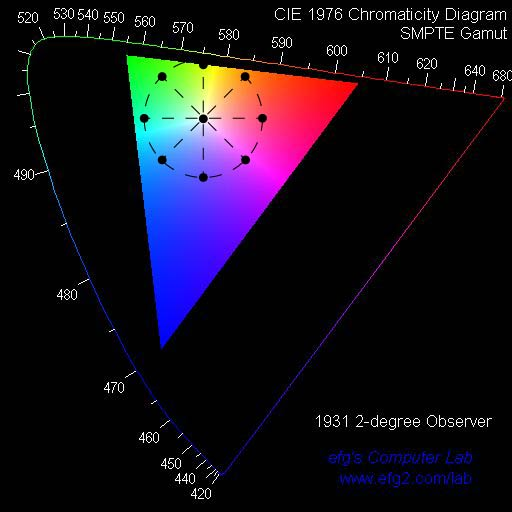
\includegraphics[width=8.0cm]{./img/CIE1976.jpg}
                    \caption{各色度の刺激の$u^{\prime}v^{\prime}Y$色度図における$u^{\prime}v^{\prime}$座標}
                    \label{uvy}
                \end{figure}

                \begin{table}[h]
                    \centering
                    \caption{15.94${\rm cd/m}^2$における各式度の刺激の$u^{\prime}v^{\prime}$座標}
                    \begin{tabular}{|l||c|c|c|c|c|c|c|c|c|} \hline
                                      & gray   & red    & orange & yellow & green  & blue-green & cyan   & blue   & magenta \\ \hline \hline
                        $u^{\prime}$  & 0.1976 & 0.2595 & 0.2452 & 0.1976 & 0.1369 & 0.1406     & 0.1505 & 0.1976 & 0.2595  \\ \hline
                        $v^{\prime}$  & 0.4699 & 0.4699 & 0.5175 & 0.5318 & 0.5307 & 0.4699     & 0.4228 & 0.4080 & 0.4080  \\ \hline
                    \end{tabular}
                    \label{uvyTable}
                \end{table}

                
            以上の工程によって得られた全ての刺激画像を図\ref{ex1_stimuli_d}と図\ref{ex1_stimuli_b}に示す.

            \begin{figure}[h]
                \centering
                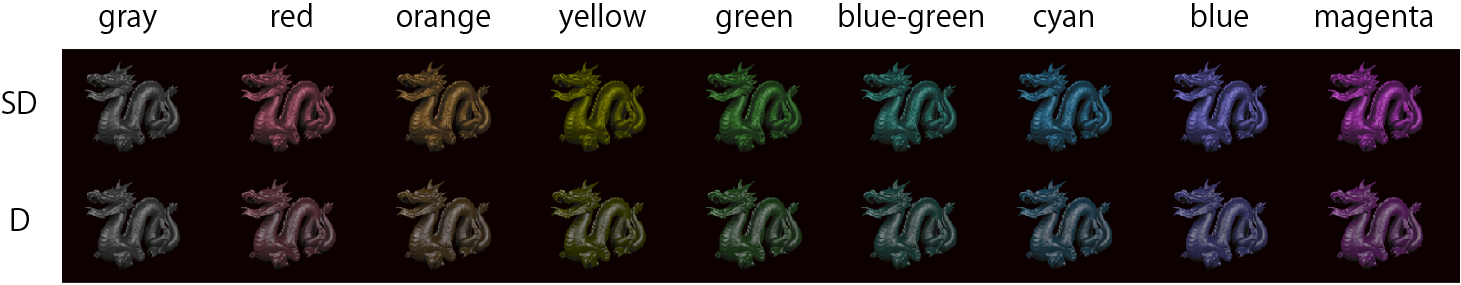
\includegraphics[width=14.0cm]{./img/ex1_stimuli_d_p.png}
                \caption{dragon形状の刺激画像}
                \label{ex1_stimuli_d}
            \end{figure}

            \begin{figure}[h]
                \centering
                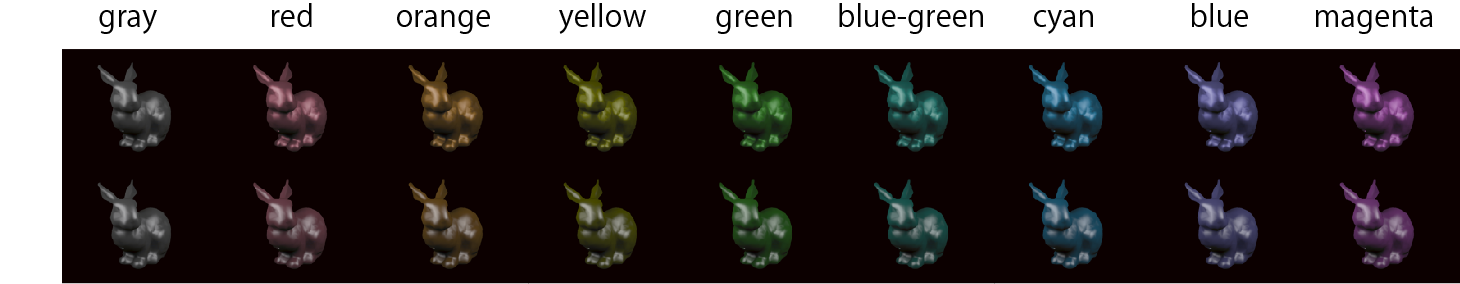
\includegraphics[width=14.0cm]{./img/ex1_stimuli_b_p.png}
                \caption{bunny形状の刺激画像}
                \label{ex1_stimuli_b}
            \end{figure}

        \subsection{実験手続き}

            \begin{figure}[h]
                \centering
                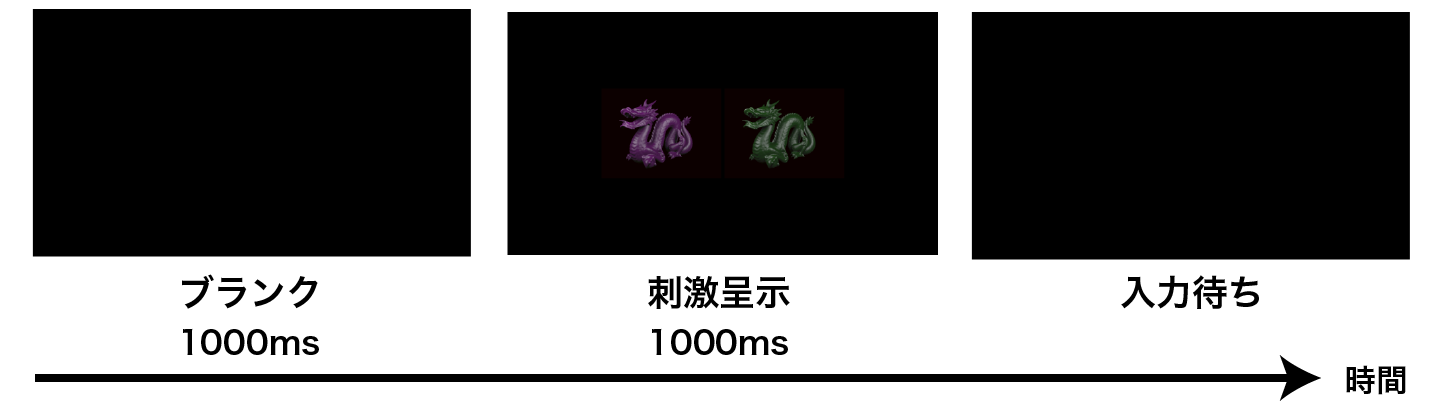
\includegraphics[width=14.0cm]{./img/ex1_procedure.png}
                \caption{1試行の流れ}
                \label{ex1_procedure}
            \end{figure}

            実験1はサーストンの一対比較法を用いて行われた.
            実験1の1試行の流れを図\ref{ex1_procedure}に示す.各試行はまず黒背景のみからなるブランク画面の1000msの呈示から始まる.
            その後,刺激対が1000msの間呈示され,その後は色順応を避けるために黒背景のみからなる入力待ち画面に移行した.
            刺激対の呈示中または入力待ち画面おいて,被験者は右画像と左画像のうちどちらからより光沢感を強く知覚するかを,マウスの左クリックまたは右クリックにより応答した.
            この後,次の試行のブランク画面に移行した.

            各セッションは2彩色条件$\times$物体形状2種類$\times$色の組み合わせ36通り=144試行から構成された.
            各被験者は全体で4セッションの実験を行った.
            各セッションの144試行で使われる刺激対は全てランダムな順序で選ばれた.
            1セッションに要する時間はおよそ8分であり,被験者は2セッション目と3セッション目の間に一度だけ休憩をとった.



    \section{実験結果}
        \subsection{解析方法}
            被験者の応答結果は,刺激同士の勝敗表としてまとめることができる.
            この勝敗表に対して,サーストンの一対比較法のケースVモデルの仮定に基づいて,応答確率のz-scoreから選好尺度値を算出した.
            次に,算出された選好尺度値を初期値とし,今度は最尤法を用いて選好尺度値を算出した.
            これを最終的な光沢感の知覚量の指標とした.
            なお,本研究で最尤法を用いた理由は,z-scoreに基づく選好尺度値の算出方法では,特に応答確率が0や1に近い刺激対においては必ず近似計算が必要となり選好尺度値の推定精度が悪化するためである.
            
        \newpage
        \subsection{各色度の刺激に対する選好尺度値}
            
            \begin{figure}[h]
                \centering
                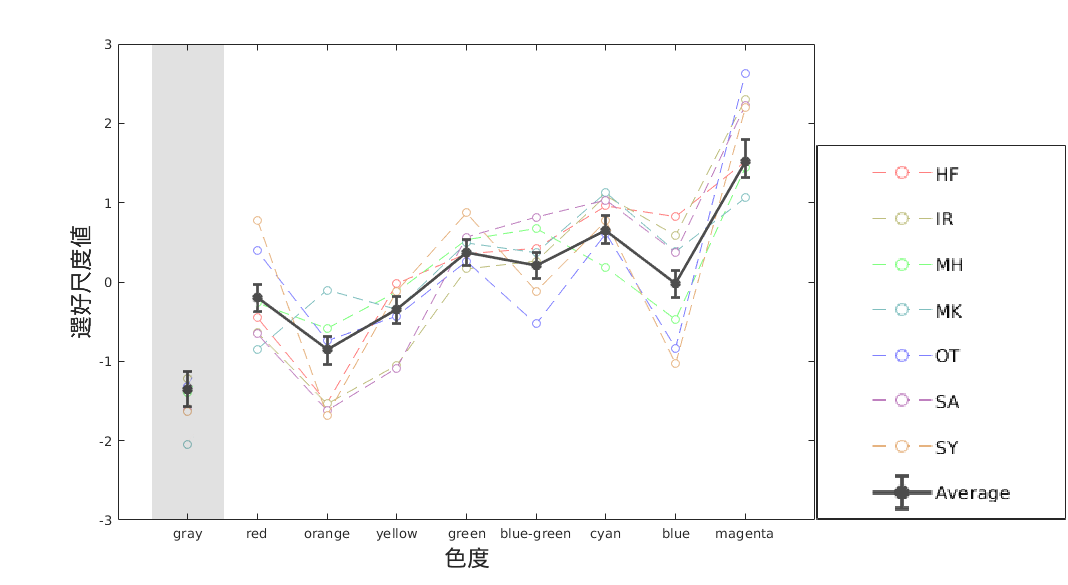
\includegraphics[width=15.0cm]{./img/ex1_res_DSD_p.png}
                \caption{Dragon形状のSD条件における選好尺度値}
                \label{ex1_DSD}
            \end{figure}

            \begin{figure}[h]
                \centering
                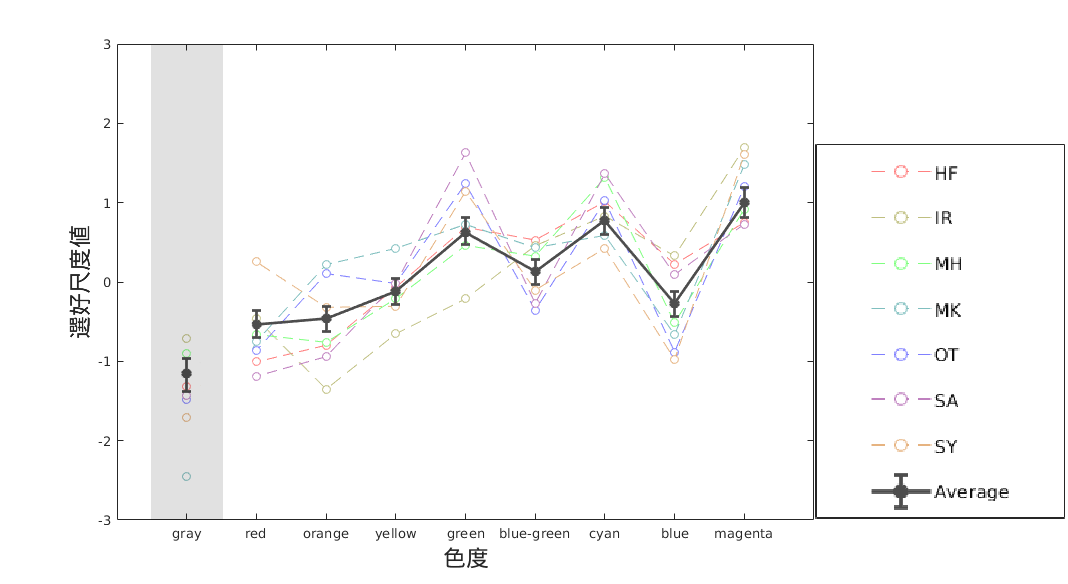
\includegraphics[width=15.0cm]{./img/ex1_res_BSD_p.png}
                \caption{Bunny形状のSD条件における選好尺度値}
                \label{ex1_BSD}
            \end{figure}
            
            \newpage
            \begin{figure}[h]
                \centering
                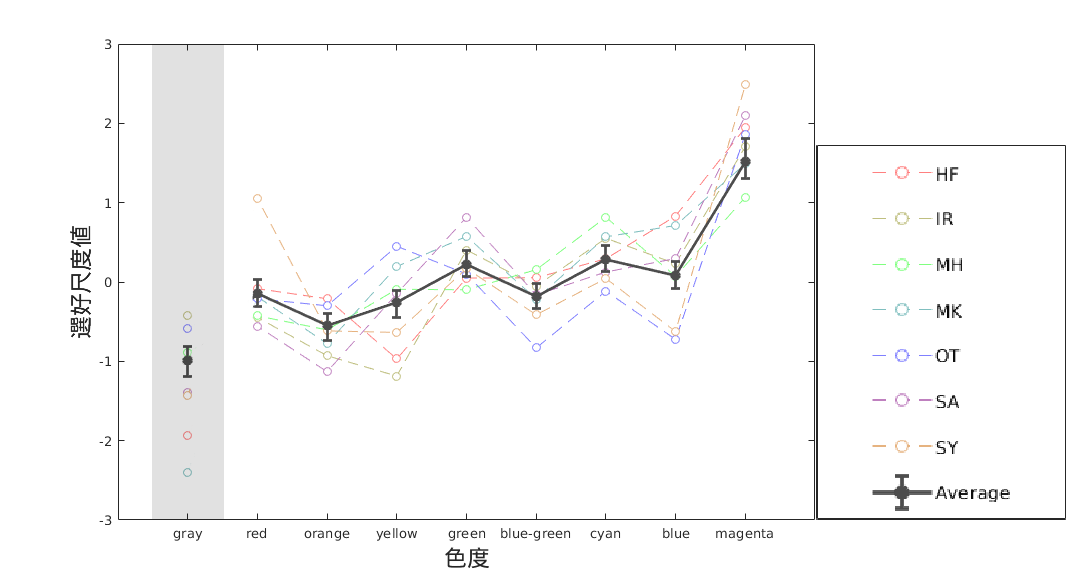
\includegraphics[width=15.0cm]{./img/ex1_res_DD_p.png}
                \caption{Dragon形状のD条件における選好尺度値}
                \label{ex1_DD}
            \end{figure}

            \begin{figure}[h]
                \centering
                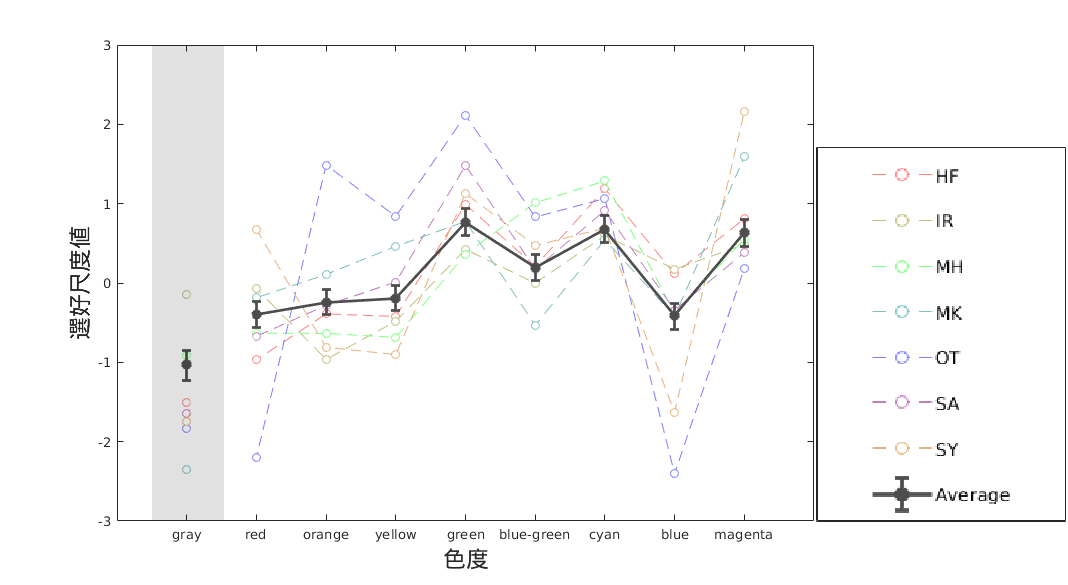
\includegraphics[width=15.0cm]{./img/ex1_res_BD_p.png}
                \caption{Bunny形状のD条件における選好尺度値}
                \label{ex1_BD}
            \end{figure}

            図\ref{ex1_DSD}から図\ref{ex1_BD}に各被験者と被験者間平均の選好尺度値を示す.
            いずれの図においても,縦軸は選好尺度値,横軸は色度の種類を表す.
            破線グラフは各被験者の結果に対応し,色は被験者の違いを表す.
            また,黒実線のグラフは被験者平均のグラフを表し,エラーバーはリサンプリング回数10000回のブートストラップ法により求められた95\%信頼区間を表す.

            これらの図では,物体形状や彩色条件に関わらず,すべての条件において色度による光沢感に違いがあった.
            統計学的にも,いずれの物体形状・彩色条件においても,リサンプリング回数10000回のノンパラメトリックブートストラップ検定によって,色度の主効果は有意であった.

            特にBunny形状のD条件を除きmagentaの光沢感が極めて高く,次いでgreen,cyanの光沢感が高いという傾向が見られた.
            また,全ての形状と条件において有彩色の光沢感は,無彩色の光沢感に比べて有意に大きかった.


            ただし,Dragon形状とBunny形状では,色度による光沢感変化の傾向に少し違いがある.
            例えば,Bunny形状のD条件では,他の3条件と比べてblueとmagentaの光沢感が比較的小さい.
            一方,Dragon形状では,他の色度に対するmegentaにおける光沢感の強さが非常に顕著に現れている.

            また,SD条件とD条件では彩色方法が大きく異なるにも関わらず,色度による光沢感変化の傾向には大きな違いはないように見える.


    \section{考察}
        本実験で最も始めに検証すべき特性は,色度による光沢感の違いの有無であった.
        実験結果では,形状やSD/D彩色条件に関わらず,色度により光沢感の有意な違いが生じた.
        この結果から,色度情報に光沢感に関する手がかりが含まれていることが明らかとなった.
        
        続いて,色度による光沢感変化に関わる視覚情報処理過程について考える.
        本実験の開始前に,色度の効果に関する作業仮説を立てていた.
        それは,鏡面ハイライトの明るさ感コントラストが光沢感の手がかりになる,という仮説であった.
        この仮説が正しければ,SD条件と比較してD条件の刺激では明るさ感コントラストが小さくなるために,D条件では色度の効果が生じにくいことが予想された.
        しかし,実験1の結果により,SD条件とD条件の応答の傾向について明確な差異はなかった.
        この結果は作業仮説を支持しないものであり,光沢感が拡散反射と鏡面反射の知覚的な明るさのコントラストによって決まっている訳ではないという可能性を示唆している.
        D条件では,たしかに鏡面ハイライトの明るさ感のコントラストは減少しているが,一方で色度コントラストは増加しており,これらの効果が相殺しあっている可能性も考えられる.
        SD条件とD条件の違いについては,第4章の総合考察で再び言及する.

        では,色度による光沢感変化はなぜ生じたのであろうか.
        ここで,orangeとyellowの光沢感が比較的小さく,magentaの光沢感が極端に大きかった点に着目する.
        これはH-K効果において,赤や青などの可視波長の端に対応する色において明るさ感が増幅されるという傾向\cite{HKeffect}の特徴と一致する.
        このことを考慮すると,H-K効果によって引き起こされた刺激全体の明るさ感の向上が,光沢感に寄与したという可能性が考えられる.

        本実験の刺激は黒背景上に呈示されていたため,特に刺激の明るさが光源色モード\cite{LightMode}としての知覚に直結しやすいと考えられることからも,刺激全体の明るさ感が光沢感に寄与した可能性も十分に考えられる.
        ところが,H-K効果の強さは測定しない限りはわからない.
        そこで,次章では本実験で用いた刺激の平均色のパッチを用いて,それらの色度に対するH-K効果の強さを測定することで,刺激全体の明るさ感が色度による光沢感増強効果を決定している可能性を検証することにする.

    \newpage